\documentclass[11pt,a4paper]{article}
\usepackage[top=2cm,bottom=2cm,left=2.2cm,right=2.2cm]{geometry}
\usepackage[T1]{fontenc}
\usepackage{newtxtext,newtxmath}
\usepackage{microtype,amsmath,booktabs,array,tabularx,xcolor,enumitem,tikz,titlesec,fancyhdr}
\usepackage[colorlinks=true,linkcolor=blue!50!black,urlcolor=blue!50!black]{hyperref}
\usetikzlibrary{arrows.meta,positioning}
\definecolor{navy}{HTML}{0B3D6B}
\titleformat{\section}{\Large\bfseries\color{navy}}{\thesection}{0.6em}{}
\titleformat{\subsection}{\large\bfseries\color{navy}}{\thesubsection}{0.6em}{}
\setlength{\parindent}{0pt}\setlength{\parskip}{5pt}
\newcolumntype{Y}{>{\raggedright\arraybackslash}X}
\pagestyle{fancy}\fancyhf{}\cfoot{\footnotesize LeakLens: the ML pipeline explained \,|\, \thepage}\renewcommand{\headrulewidth}{0pt}
\newcommand{\code}[1]{\texttt{#1}}
\begin{document}
\begin{center}
{\Huge\bfseries\color{navy} LeakLens}\\[3pt]{\large Water Leak Localization System}\\[8pt]
{\LARGE The ML Pipeline, Explained}\end{center}
\hrule\vspace{3mm}

The pipeline is mostly \textbf{physics-based processing in front of a small machine-learning model}. Only the ``which cause?'' step is learned from data. The noise levels, the leak ranking and the quiet check are calculations, not trained models. All results are from simulation, not real sensors.

\begin{center}
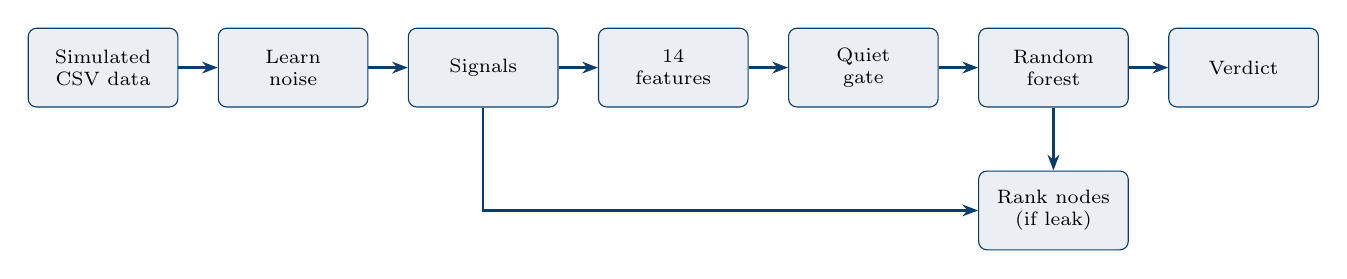
\begin{tikzpicture}[node distance=5mm,
 box/.style={draw=navy,fill=navy!8,rounded corners=3pt,minimum width=1.9cm,minimum height=1.0cm,align=center,font=\scriptsize},
 arr/.style={-{Stealth[length=2mm]},thick,navy}]
\node[box](a){Simulated\\CSV data};
\node[box,right=of a](b){Learn\\noise};
\node[box,right=of b](c){Signals};
\node[box,right=of c](d){14\\features};
\node[box,right=of d](e){Quiet\\gate};
\node[box,right=of e](f){Random\\forest};
\node[box,right=of f](g){Verdict};
\node[box,below=8mm of f](h){Rank nodes\\(if leak)};
\draw[arr](a)--(b);\draw[arr](b)--(c);\draw[arr](c)--(d);\draw[arr](d)--(e);\draw[arr](e)--(f);\draw[arr](f)--(g);\draw[arr](f)--(h);\draw[arr](c.south)|-(h.west);
\end{tikzpicture}
\end{center}
Code lives in \code{ml\_pipeline/}: \code{dataset.py}, \code{features.py}, \code{detector.py}, \code{classifier.py}, \code{localizer.py}, \code{pipeline.py}, \code{train.py}, \code{evaluate.py}.

\section{Training and testing: the 80/20 split (\code{split.py})}
If a system is tested on the scenarios it learned from, it looks perfect and tells us nothing. So all 617 scenarios were split once (fixed seed) into \textbf{478 for learning (about 80\%)} and \textbf{139 for testing (about 20\%)}.
\begin{itemize}[itemsep=2pt]
\item \textbf{Learned from training scenarios only:} the noise thresholds and the random forest.
\item \textbf{Measured on test scenarios only:} every result in this document. The system never saw them while learning.
\item \textbf{Near-copies stay together:} all leaks at the same junction (every size, start time, noise and ``hidden behind'' variant), and a scenario with its noisy twin, are on the same side. Otherwise the test would be too easy.
\item \textbf{Stratified:} each network and each kind of event is split about 80/20. The test set has 12 scenarios of every non-leak kind and 67 leaks.
\item The dashboard tags every scenario \emph{Unseen test} or \emph{Training}.
\end{itemize}

\section{Data in (\code{dataset.py})}
\begin{itemize}[itemsep=2pt]
\item Each scenario has three tables with one row per hour: \textbf{node pressure}, \textbf{pipe flow} and \textbf{metered node demand}. Each network also has a normal-day baseline.
\item The network layout is read from the EPANET file. From it we build a \textbf{pipe graph} (nodes joined by pipes, with lengths) and an \textbf{incidence matrix}, so inflow minus outflow at every node is one matrix multiplication.
\item Unreliable readings are dropped: Net3 nodes 61 and 601 and hour 21 swing wildly for a 1\% demand change (pump switching).
\end{itemize}

\section{Learn what noise looks like (\code{features.py: calibrate})}
Each network has 18 \emph{normal runs} that contain only sensor noise; only the training ones (about 14 per network) are used. From them the system learns the noise level of pressure, of each pipe's flow, of each node's demand and of each node's unaccounted flow. The pressure threshold is
\[\tau_P=\max\{0.1\ \text{m},\;4\,\sigma_P\}\approx 0.5\ \text{m}\]
in all three networks. Every later signal is divided by its noise level, so ``1.0'' means ``right at the noise limit''. This lets one set of features work on networks of different size.

\section{Build signals (\code{features.py: node\_signals})}
\textbf{Pressure drop.} $r_i(t)=P^{\text{normal}}_i(t)-P^{\text{obs}}_i(t)$. It only counts if it stays high for two consecutive hours: $d_i=\max_t\min\{r_i(t),r_i(t{+}1)\}$. One noisy reading cannot trigger anything.

\textbf{Unaccounted flow.} With pipe flows signed $+1$ into and $-1$ out of node $i$,
\[u_i(t)=\sum_p\operatorname{sign}(p,i)\,\Delta Q_p(t)\;-\;\Delta D_i(t)\;=\;Q_{\ell,i}(t).\]
In noise-free data this is exactly the leak flow at node $i$ and zero elsewhere. A demand change cancels because it is metered.

\section{Fourteen features (\code{features.py: extract})}
One row of 14 numbers per scenario. Flows are divided by total customer demand, so networks of different size give comparable numbers.
\begin{center}\small\begin{tabularx}{\linewidth}{@{}>{\bfseries}p{3.0cm}>{\ttfamily}p{3.6cm}Y@{}}\toprule
Group & Features & Meaning \\\midrule
Pressure drops & drop\_ratio, frac\_hit, median\_ratio, conc\_drop & largest drop, share of junctions affected, typical drop, is it centred on one node \\
Pressure rises & rise\_ratio, frac\_rise & some nodes gain pressure (as with blockages) \\
Pipe flows & flow\_frac & share of pipes with changed flow \\
Sources & source\_change, tank\_change, pump\_drop & reservoir supply change, tank flow change, pump flow lost (1 = off) \\
Leak evidence & unacc\_ratio, unacc\_conc & largest unaccounted flow, its concentration at one node \\
Demand evidence & demand\_frac, demand\_total & share of nodes with changed metered demand; total change \\\bottomrule\end{tabularx}\end{center}

\section{Stage 1: the quiet gate (\code{quiet\_mask})}
If $\text{drop\_ratio}<1$, $\text{rise\_ratio}<1$, $\text{unacc\_ratio}<1$, $\text{flow\_frac}<0.1$ and $\text{demand\_frac}=0$, the answer is \textbf{normal} and nothing more runs. This removes false alarms from sensor noise. It is also why tiny leaks are reported as normal.

\section{Stage 2: the classifier (\code{classifier.py}, \code{train.py})}
\begin{itemize}[itemsep=2pt]
\item \textbf{Model:} a scikit-learn \textbf{random forest}: 300 decision trees voting, \code{class\_weight="balanced"}, \code{random\_state=0}. ``Balanced'' matters because leaks are about half the scenarios; it keeps the rarer classes from being ignored.
\item \textbf{Training data:} 478 rows (the training scenarios), one per scenario. The label is the true event class: normal, leak, demand change, pump/reservoir, tank, blocked pipe, ageing.
\item \textbf{Interpretable twin:} a depth-4 decision tree is also trained; its readable rules are saved to \code{data/results/decision\_rules.txt}.
\item \textbf{Output:} a probability for each class. The highest is the verdict; its probability gives the High / Medium / Low confidence label (85\% and 60\% cut-offs).
\item Hyperparameters were \emph{not} tuned.
\end{itemize}

\section{Localization (\code{localizer.py})}
Only runs when the verdict is ``leak''. For each junction, with $A_i=u_i^{\text{peak}}/\max_ju_j^{\text{peak}}$ and $D_i=d_i/\max_jd_j$,
\[S_i=A_i+0.3\,D_i .\]
Nodes are sorted by $S_i$; the first is the Top-1 prediction. Error is the number of pipes (and metres) between the predicted and the true node. This step is \emph{not trained}. Smoothing the scores over neighbouring nodes was tested and gave no improvement on the test leaks, so it is off.

\section{How it is checked (\code{evaluate.py})}
\begin{itemize}[itemsep=2pt]
\item \textbf{Cause classification:} fitted on the training scenarios, scored on the 139 test scenarios. Also \textbf{leave-one-network-out}: train on the training scenarios of two networks, test on the third network's test scenarios.
\item \textbf{Detection:} compared with the old fixed 0.5 m alarm, on the test scenarios.
\item \textbf{Localization:} the 60 scored test leaks, compared with the first version, with and without demand meters, and pressure only.
\item Training-set numbers are also computed, only to show the gap; time per scenario is about 22 ms.
\end{itemize}
\begin{center}\small\begin{tabular}{@{}lcc@{}}\toprule
Result on unseen test scenarios & First version & Final \\\midrule
Leak exact node ranked first (Top-1, 60 leaks) & 58.3\% & \textbf{96.7\%} \\
Real leak in first five nodes (Top-5) & 71.7\% & \textbf{98.3\%} \\
False alarms on normal test days (12 days) & 41.7\% & \textbf{0.0\%} \\
Right cause identified (139 test scenarios) & --- & \textbf{82.7\%} \\
Right cause on the training scenarios, for comparison & --- & 95.6\% \\\bottomrule\end{tabular}\end{center}

\section{Weak points to know}
\begin{itemize}[itemsep=3pt]
\item The model is \textbf{small and cheap}: 14 features, 478 training rows, no tuning.
\item The \textbf{test set is small}: 139 scenarios, only 60 scored leaks (one miss is about 1.7 points) and 12 normal days. Percentages have wide margins of error, and the split was made once.
\item \textbf{Settings chosen earlier:} the ranking weight (0.3) and the quiet-gate cut-offs were chosen while looking at all scenarios, before the split existed. They were not re-tuned afterwards.
\item \textbf{Training versus test gap:} cause accuracy is 95.6\% on training and 82.7\% on test, a sign the model partly memorises. Pump, tank, blockage and ageing are mixed up with each other most.
\item \textbf{Unseen network:} leaks are mostly found, but accuracy for causes falls to 49--82\%, and without demand meters to about 15\% on Net3.
\item It \textbf{relies on demand meters}. Leaks inside the sensor noise are reported as normal.
\item The dashboard's confidence for a \emph{training} scenario is optimistic; use the Unseen test tag.
\item All of this is simulation, not real sensor data.
\end{itemize}
\end{document}
